El ``Plan estratégico de la Universidad de Talca Visión 2020'' destaca el apoyo a todo tipo de actividades emprendidas por las distintas Organizaciones Estudiantiles reconocidas. Entre las actividades destacan: recepción de alumnos nuevos; celebración del día de la carrera; actividades sociales, culturales y deportivas; entre otras~\cite{5}.

%\begin{figure}[!p]
%  \vspace*{1cm}
%  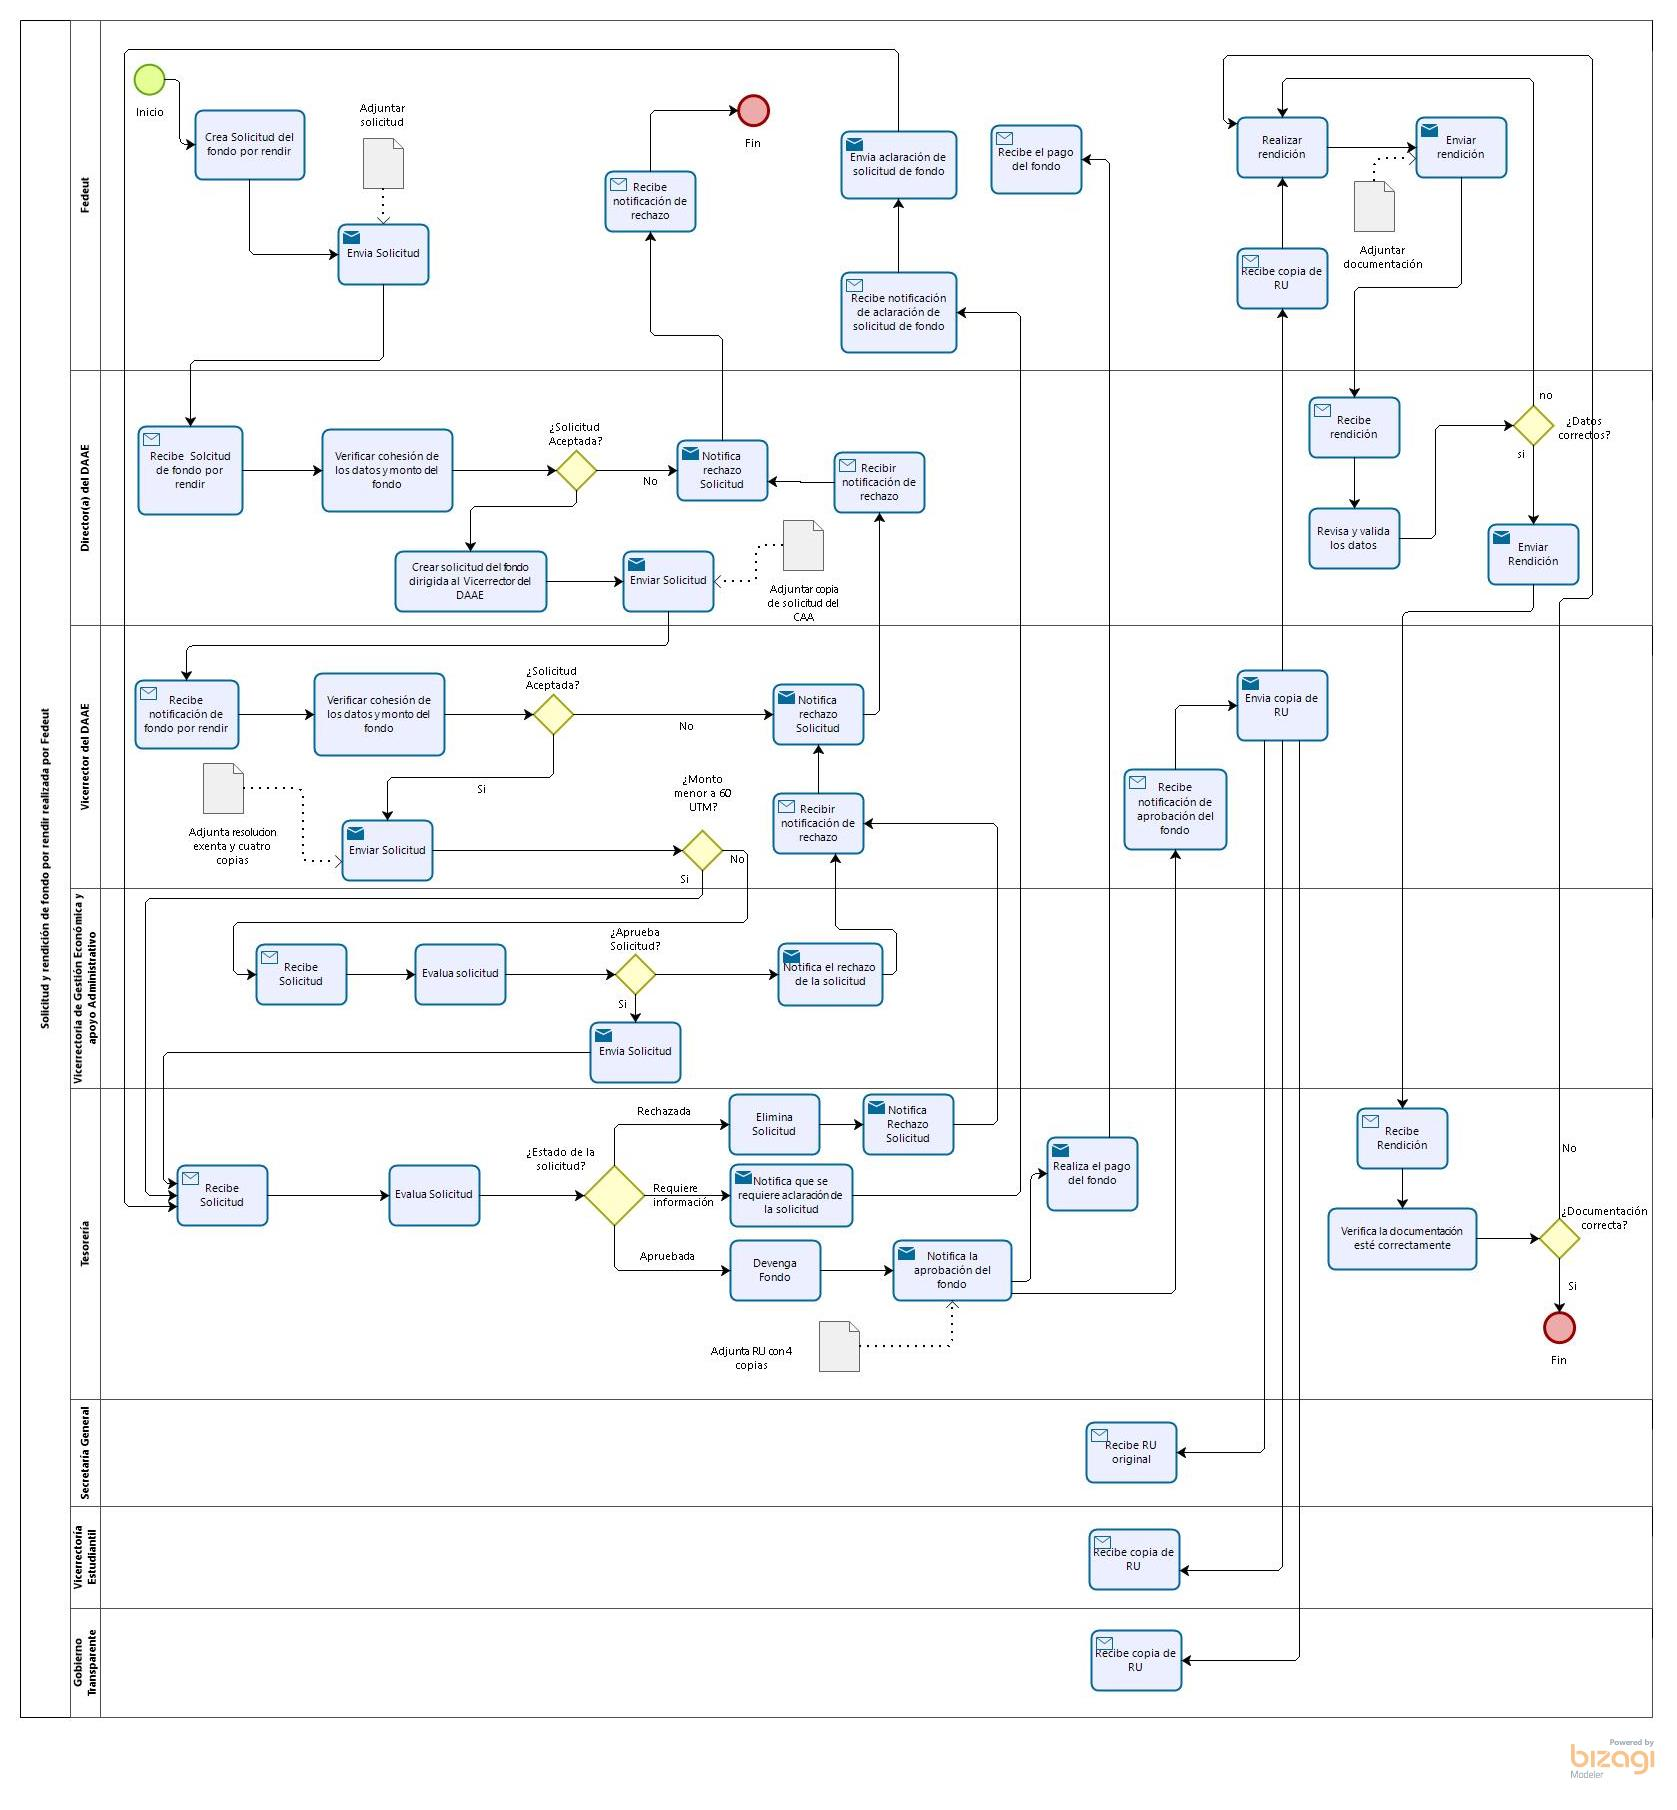
\includegraphics[bb=0 0 640 480, width=.5\linewidth]{Imagenes/Solicitud_Federacion.jpg}
%  \vspace*{1cm}
%  \caption{\label{fig: Solicitud_Federacion}Proceso de Fondos por Rendir por parte de Fedeut.}
%\end{figure}

\begin{figure}[p!]
    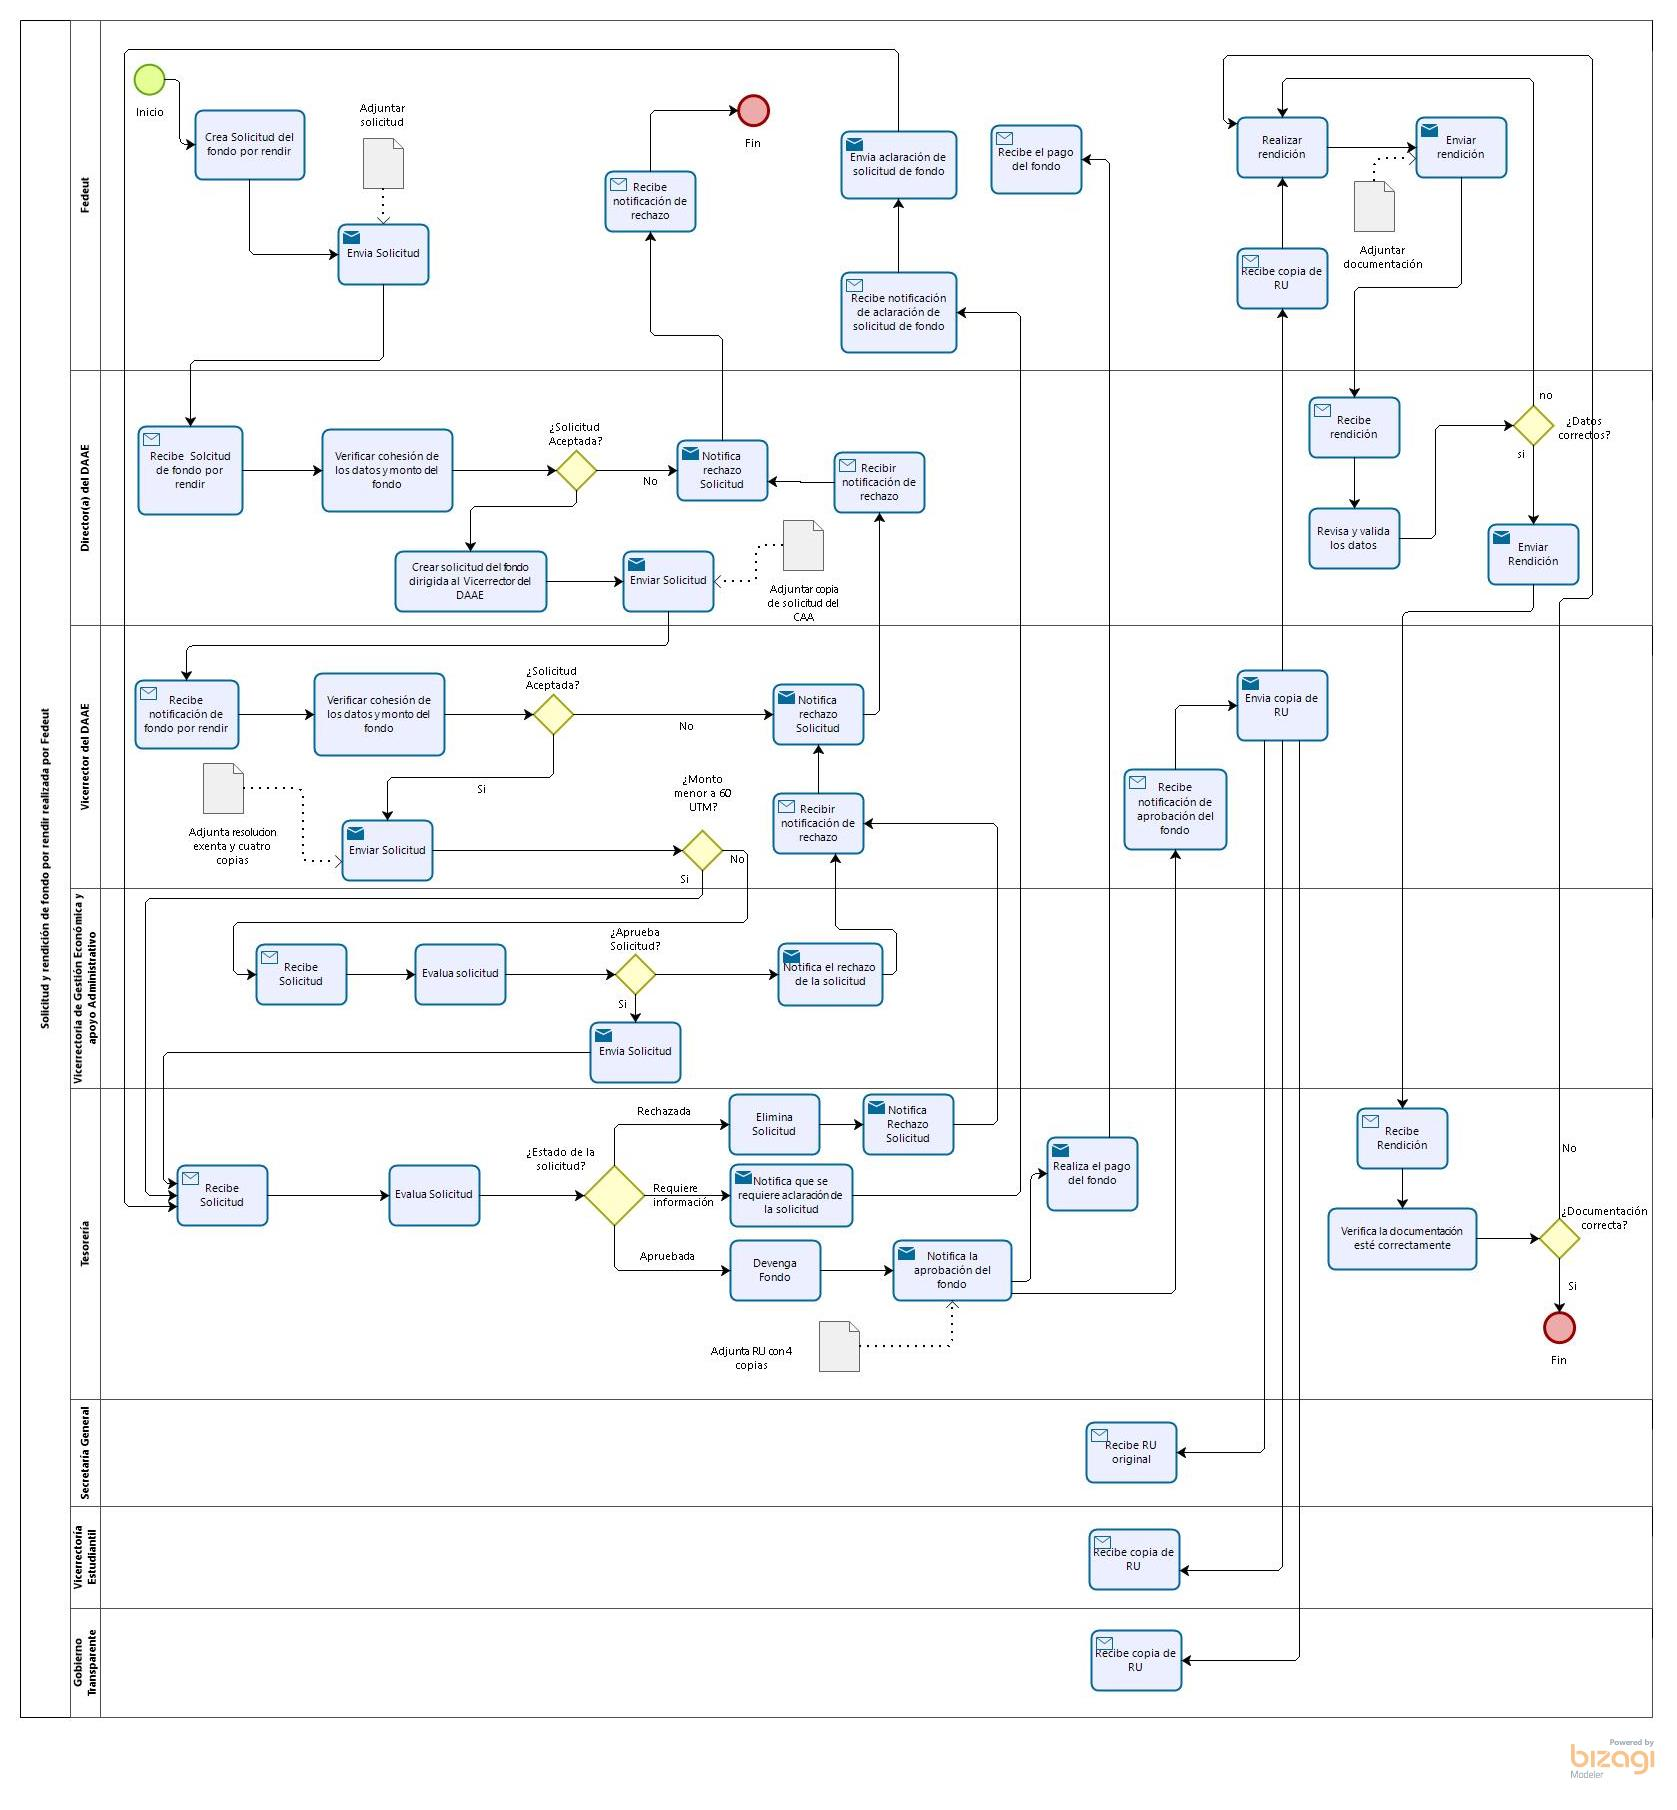
\includegraphics[width=\textwidth]{Imagenes/Solicitud_Federacion.jpg}
    \caption{\label{fig: Solicitud_Federacion}Proceso de Fondos por Rendir por parte de Fedeut.}
\end{figure}

Para la realización de estas actividades se debe seguir un procedimiento, el cual está estipulado en la RU N\grad 2083 promulgada el 12 de diciembre del 2017, la cual dice:

\begin{tasks}[counter-format = {tsk[A].}]
    \task \textbf{Caso Federación y Organizaciones Estudiantiles:}

    Sólo el Presidente, Tesorero o Secretario de finanzas de la Federación (Fedeut) o uno de Grupos Intermedios pueden solicitar por escrito Fondos para realizar actividades. Esta solicitud se envía a quien dirige la Dirección de Apoyo a Actividades Estudiantiles (DAAE), de la Vicerrectoría de Desarrollo Estudiantil (VDE), al menos 20 días antes del inicio de la actividad. 

    Quien dirige la DAAE, una vez que verifica la solicitud enviada por Fedeut o Grupo Intermedio y una vez aprobada, realiza y envía otra solicitud a quien dirige la VDE.

    Luego de que quien dirige la VDE verifica y aprueba la solicitud de Fondo, emite una Resolución Exenta en original y cuatro copias las cuales son enviadas a Contraloría de la Universidad de Talca para su respectivo control de legalidad. 
    
    Una vez tramitado el acto administrativo, se debe distribuir los documentos anteriormente mencionados de la siguiente forma: 

    \begin{itemize}
        \item La documentación original la archiva Secretaría General.
        \item La primera copia es enviada al Departamento de Tesorería y Presupuesto.
        \item La segunda para el archivo de la Vicerrectoría Estudiantil.
        \item La tercera es enviada a la Federación o Grupo Intermedio interesada.
        \item La cuarta es enviada a la Unidad de Gobierno Transparente.
    \end{itemize}

    Este proceso se puede apreciar con mayor detalle en la \textbf{Figura \ref{fig: Solicitud_Federacion}}.

    \task \textbf{Caso de Centros de Alumnos}

    Sólo el Presidente, Tesorero o Secretario de finanzas del Centro de Alumnos (CAA) pueden solicitar por escrito Fondos para realizar actividades. Esta solicitud se envía a quien dirige la Dirección de Escuela correspondiente al menos 20 días antes del inicio de la actividad. 

    Quien dirige la Dirección de Escuela, una vez que verifica la solicitud enviada por el CAA, eleva la solicitud a quien dirige la Decanatura de la Facultad o a quien dirige la Vicerrectoría de Desarrollo Estudiantil (para el caso de las Escuelas no adscritas a una Facultad).

    Luego de que quien dirige la Decanatura de la Facultad o Vicerrectoría de Desarrollo Estudiantil según corresponda, verifique y apruebe la solicitud de Fondo enviada por quien dirige la Dirección de Escuela, emite una Resolución Exenta, en original y cuatro copias, las cuales son enviadas a controlaría universitaria para el respectivo control de legalidad.

    Una vez aprobada por Contraloría Interna y totalmente tramitada, es enviada a quien dirige Decanatura o VDE para su distribución de la siguiente forma: 
    \begin{itemize}
        \item La documentación original la archiva Decanato o VDE.
        \item La primera copia es enviada al Departamento de Tesorería y Presupuesto.
        \item La segunda para el archivo de la Facultad.
        \item La tercera es enviada al CAA interesado.
        \item La cuarta es enviada a la Unidad de Gobierno Transparente.
    \end{itemize}

    Se puede apreciar con mayor detalle en la \textbf{Figura \ref{fig: Solicitud_CAA}}.

\end{tasks}

\begin{figure}[p!]
    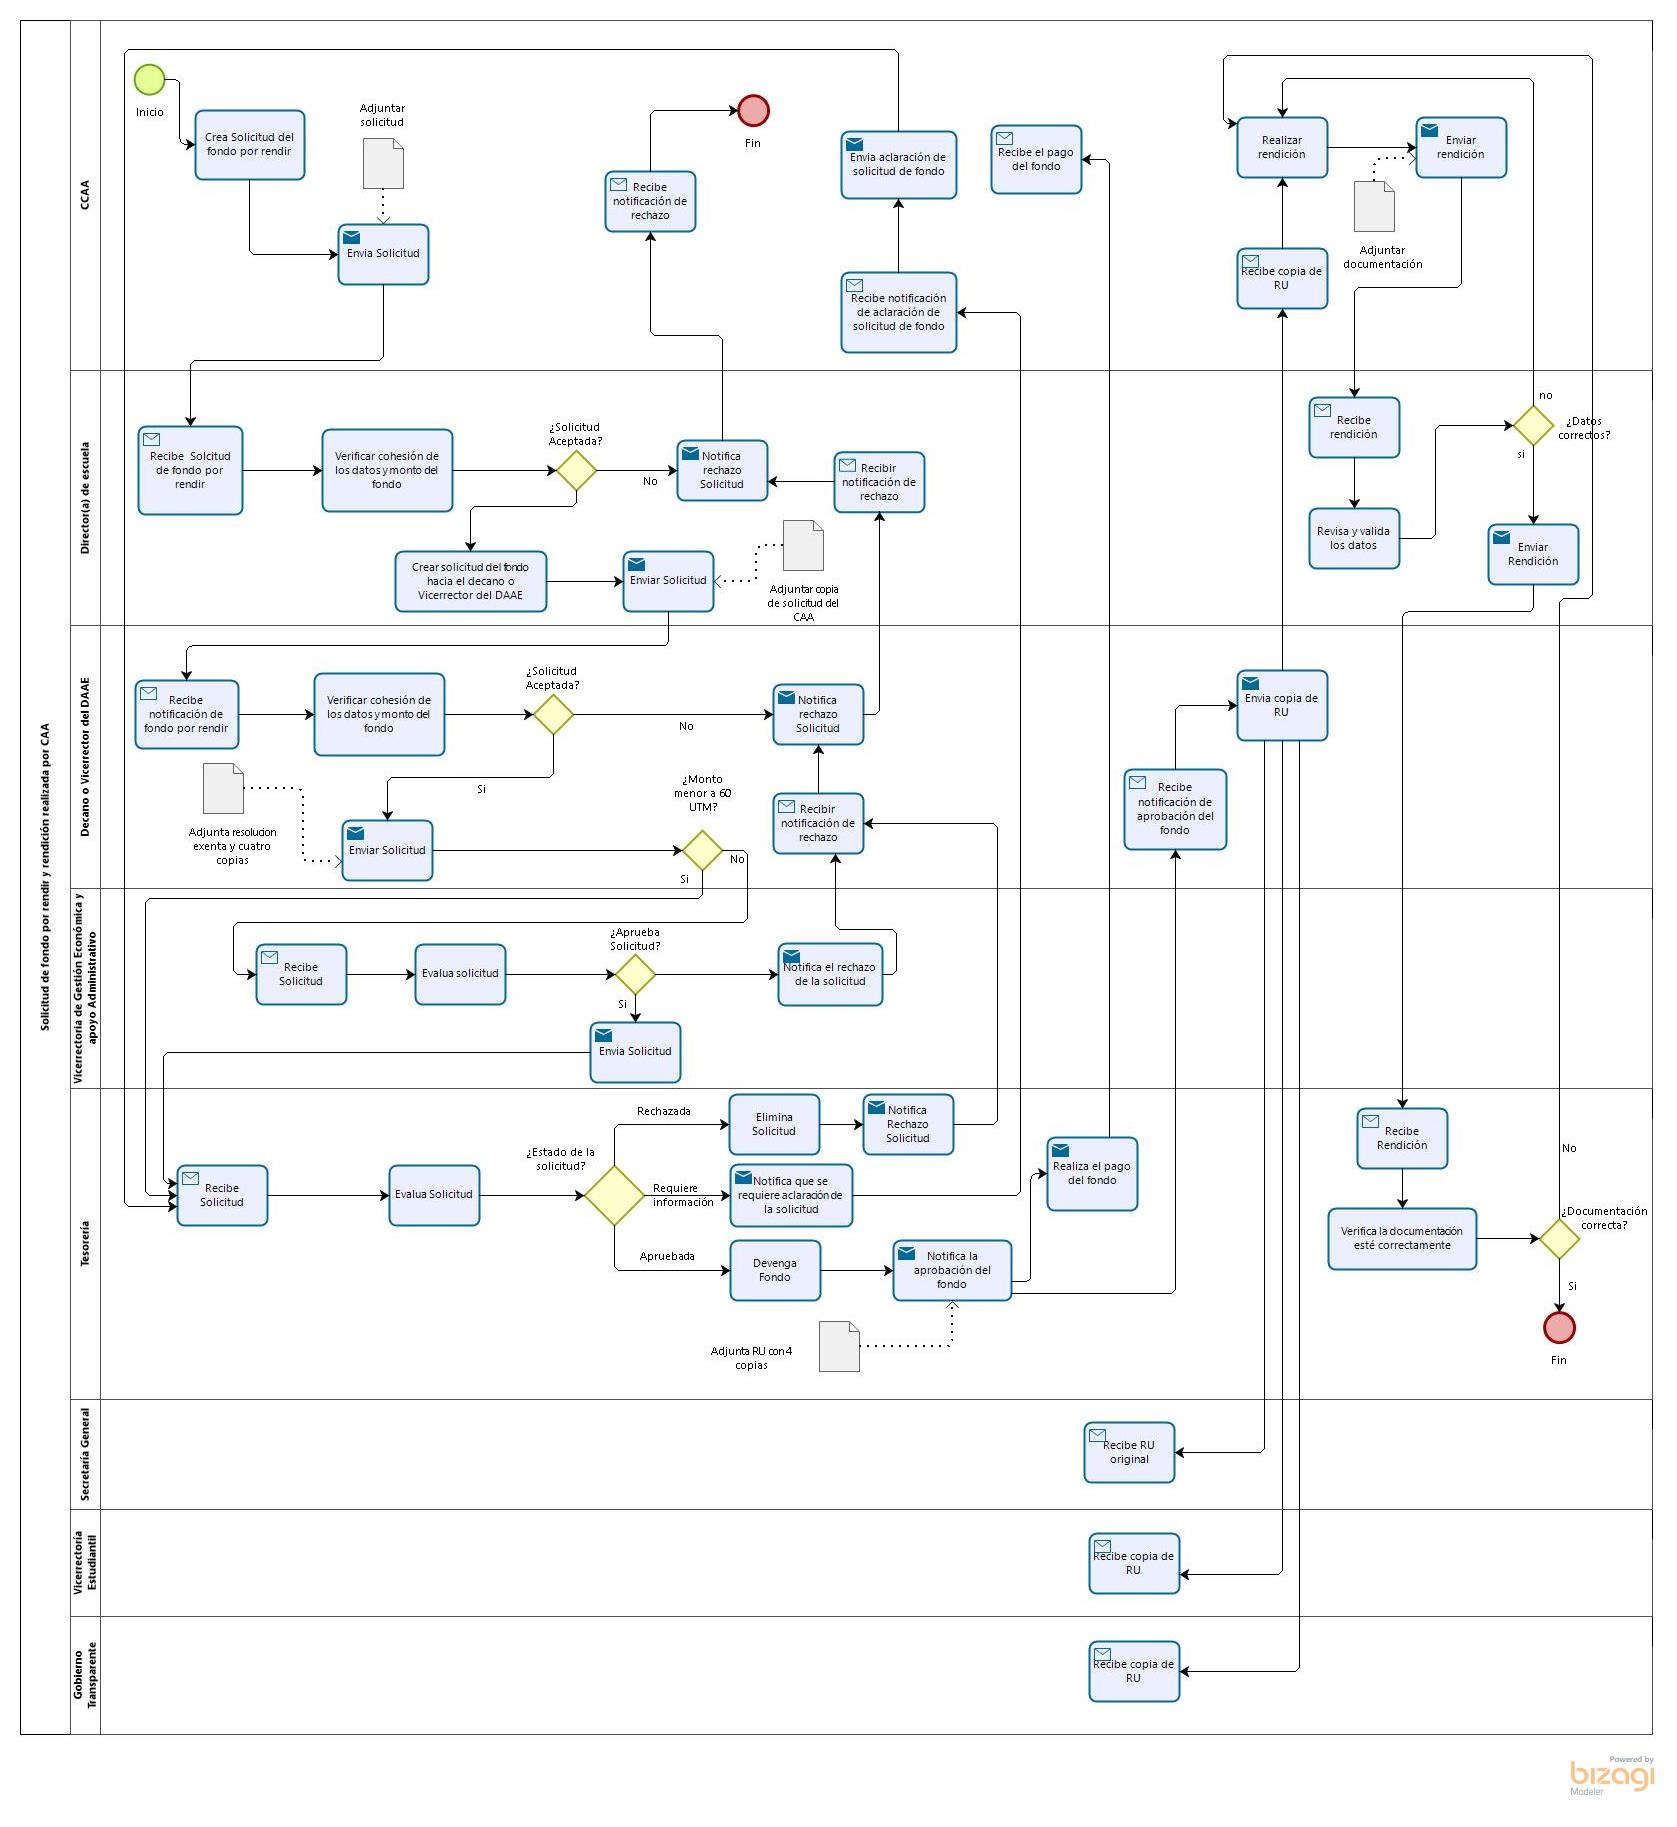
\includegraphics[width=\textwidth]{Imagenes/Solicitud_CCAA.jpg}
    \caption{\label{fig: Solicitud_CAA}Proceso fondos por rendir por parte de CAA.}
\end{figure}

En ambos casos, el Departamento de Presupuesto hace responsable de la actividad presupuestaria correspondiente a la O.E. (ya sea Fedeut, CAA o Grupo Intermedio) que la solicita.

El Departamento de Tesorería emite el pago a nombre del Presidente, Tesorero o Secretario de Finanzas de la O.E. y adjunta la segunda copia de la Resolución al Comprobante de Egreso para la posterior rendición del Fondo.

Al representante de la O.E. se le asigna las siguientes responsabilidades:

\begin{itemize}
    \item Supervisar o realizar el cobro del documento de pago.
    \item Mantener un registro detallado de los gastos establecidos en el presupuesto de la actividad aprobada.
    \item Ejecutar/Realizar los gastos autorizados para la actividad.
    \item Rendir el Fondo asignado para la actividad.
    \item Respaldar gastos con la documentación idónea, tal como establece la Resolución Universitaria N\grad 522 de 1992, punto N\grad 12. 
\end{itemize} 